\graphicspath{{chapters/13/images/}}
\chapter{The grand canonical ensemble}

\section{Introduction}
The Gran Canonical (GC) ensemble comes in handy when we cannot keep the molecules fixed in the simulations. 
This is one of the main differences between MD and MC approaches: it is not possible to perform MD simulations with varying number of molecules.
	\subsection{Euler's theorem}
	
	Homogeneous function $f(x_1, \dots, x_N)$ of degree $n$ in $x_1, \dots, x_k$:

	$$f(\lambda x_1, \dots, \lambda x_k, x_{k+1}, \dots, x_N) = \lambda^n f(x_1, \dots, x_k, \dots, x_N)$$
	
	This property states that if each variable $(x_1, ... x_k)$ is \textit{increased} by a certain value $\lambda$, then the net result is that the value of the function is increased by a factor $\lambda^n$.
	
	An example of this property can be showed by the homogeneous function $f(x) = x^2$, $f(x, y, z) = xy^2+z^3$.
	The degree is $3$ and each variable $(x, y, z)$ is increased by a factor $\lambda$. 
	
	We can also easily take the derivative:
	$$\frac{d}{d\lambda} f(\lambda x_1, \dots, \lambda x_k, \dots, x_N) = n\lambda^{n-1}f(x_1, \dots, x_k,\dots, x_N)$$
	
	If the partial derivative is calculated wrt each variable and then the derivative of the variable itself wrt $\lambda$, it is obtained:
	
	$$\frac{d}{d\lambda}f(\lambda x_1, \dots, \lambda x_k, \dots, x_N) = \sum\limits_{i=1}^k\frac{\partial f(x_1, \dots, x_k, \dots, x_N)}{\partial x_i}x_i$$

Meaning, the two quantities are equal and we can derive the following property (for an homogeneous function):

	$$\lambda = 1 \Rightarrow \sum\limits_{i=1}^k\frac{\partial f}{\partial x_i}x_i = nf(x_1, \dots, x_N)$$

	\subsection{Applications}
	
	Euler's theorem has important consequences in thermodynamics, as it means that we can express all of the thermodynamics function in terms of other parameters, and it is valid for every substance.
	Let's apply Euler's theorem to the internal energy $U$: 

	$$U(\lambda N, \lambda V, \lambda S) = \lambda U(N, V, S)\Rightarrow U(N, V, S) = \frac{\partial U}{\partial N}N + \frac{\partial U}{\partial V}V_\frac{\partial U}{\partial S}S = \mu N - PV + TS$$
	
	Each of the above partial derivatives are easily calculated through Maxwell square.
	Let's apply the theorem to Helmholtz free energy:

	$$A(\lambda N, \lambda V, T) = \lambda A(N, V, T) \Rightarrow A(N, V, T) = \frac{\partial A}{\partial N}N + \frac{\partial A}{\partial V}V = \mu N - PV$$

The difference here is that the extensive quantities are $N$ and $V$, while $T$ is an intensive quantity.  
The function is not homogenous in $T$, e.g. if T is increased by a factor $\lambda$ the whole function is not increased.

Let's apply now to the enthalpy:

	$$H(\lambda N, \lambda S, P) = \lambda H(N, S, P)\Rightarrow H(N, S, P) = \frac{\partial H}{\partial N}N+\frac{\partial H}{\partial N}N+\frac{\partial H}{\partial S}S = \mu N+TS$$
	
	Like for $A$, the enthalpy is a homogenous function for two of its variables, but not for $P$.
	Finally, the Gibbs free energy:

	$$G(\lambda N, P, T) = \lambda G(N, P, T)\Rightarrow G(N, P, T) = \frac{\partial G}{\partial N}N= \mu N$$

It has only one dependency on an extensive quantity: the number of particles. 
We can also retrieve the fact that the chemical potential $\mu$ is exactly $G$ divided by $N$, as demonstrated in the previous chapter. 

	\subsection{Legendre transform of A}
	Let's apply the same reasoning that was applied to the isobaric ensembles:

	$$\tilde{f}(s) = f(x(s))-sx(s)\qquad s = f'(x)$$

	The legendre transform will not be applied in terms of volume, but instead in terms of its derivative wrt number of molecules:
	
	\begin{align*}
		\tilde{A}\biggl(\frac{\partial A}{\partial N}, V, T\biggr) &= A(N(\mu), V, T)-\biggl(\frac{\partial A}{\partial N}\biggr)_{N, V}N\biggl(\frac{\partial A}{\partial N}, V, T\biggr) = \\
																															 &=A(N(\mu), V, T) - \mu N = \mu N - PV - \mu N = -PV
	\end{align*}
	From the results obtained before, the result of the legendre transform is simply $-PV$. 
	
	We need now to calculated the infinitesimal variation of the transformed $A$:
	$$d\tilde{A} = dA - Nd \mu -\mu dN = -PdV - SdT + \mu dN -Nd\mu - \mu dN$$

	$$d\tilde{A} = -PdV - SdT - Nd\mu$$

	$$\tilde{A}(\mu, \lambda V, T) = \lambda\tilde{A}(\mu, V, T)\Rightarrow \tilde{A}(\mu, V, T) = \frac{\partial \tilde{A}}{\partial V}V = -PV$$
	
	Notice that $\tilde{A}$ depends on only one extensive variable ($V$), so Euler's theorem can be applied again.
	
	
\section{Grand canonical ensemble}
As for the previous ensembles, the analysis starts from the definition of the main variables of the equations and in figure \ref{fig:grand} the two systems are depicted. 

\begin{figure}
\center
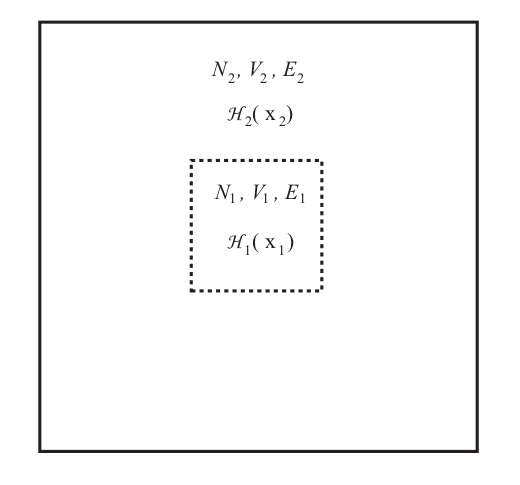
\includegraphics[scale=0.5]{grand.png}
\caption{Two systems in contact with a common thermal reservoir at temperature $T$. System $1$ has $N_1$ particles in a volume $V_1$ ; system 2 has $N_2$ particles in a volume $V_2$. The dashed lines indicate that systems $1$ and $2$ can exchange particles.}
\label{fig:grand}
\end{figure}

\begin{multicols}{2}
	\begin{itemize}
		\item $E = E_1 + E_2\quad E_2\gg E_1$.
		\item $N = N_1 + N_2\quad N_2\gg N_1$.
		\item $V = V_1 + V_2\quad V_2\gg V_1$.
		\item $\mathcal{H}(x, N) = \mathcal{H}_1(x_1, N_1) + \mathcal{H}_2(x_2, N_2)$.
	\end{itemize}
\end{multicols}

The partition function is the same as a canonical ensemble, if we stop the exchange of molecules between the two systems.

$$Q(N, V, T) = \frac{1}{N!h^{3N}}\int dx_1\int dx_2e^{-\beta[\mathcal{H}_1(x_1) + \mathcal{H}_2(x_2)]}$$

At fixed $N_1$ and $N_2$, not allowing any other exchange of particles, then the partition function is:

$$Q(N, V, T) = \frac{N_1!N_2!}{N!}\frac{1}{N_1!h^{3N_1}}\int dx_1 e^{-\beta\mathcal{H}_1(x_1)}\frac{1}{N_2!h^{3N_2}}\int dx_2^{-\beta\mathcal{H}_2(x_2)} = \frac{N_1!N_2!}{N!}Q_1(N_1, V_1, T)Q_2(N_2, V_2, T)$$

With a varying particle numbers:

$$Q(N, V, T) = \sum\limits_{N_1=0}^Ng(N_1, N-N_1)\frac{N_1!(N-N_1)!}{N!}Q_1(N_1, V_1, T)Q_2(N-N_1, V-V_1, T)$$

The factor $g$ is a combinatorial (or degeneracy) factor, and indicates in how many ways the particles can be divided in one box and the other, or in how many ways there are $N_1$ particles in system $1$ and $N_2$ particles in system $2$.
It is defined as:
$$g(N_1, N-N_1) = \frac{N!}{N_1!(N-N_1)!}$$

\begin{multicols}{3}
	\begin{itemize}
		\item $N_1 = 0\Rightarrow g(0, N) = 1$.
		\item $N_1 = 1\Rightarrow g(1, N-1) = N$.
		\item $N_1 = 2\Rightarrow g(2, N-2) = \frac{N(N-1)}{2}$.
	\end{itemize}
\end{multicols}

So the total partition function is defined as:

$$Q(N, V, T) = \sum\limits_{N_1=0}^NQ_1(N_1, V_1, T)Q_2(N-N_1, V-V_1, T)$$

However for the full system, considered as a canonical ensemble we know the partition function:

$$f(x, N) = \frac{e^{-\beta\mathcal{H}(x, N)}}{N!h^{3N}Q(N, V, T)}\Rightarrow dxf(x, N) = 1$$

And the phase space distribution of system $1$: $\sum\limits_{N_1=0}^{N}\int dx_1f(x_1, N_1) = 1$.

\begin{align*}
	f(x_1, N_1) &=\biggl(\frac{e^{-\beta\mathcal{H}_1(x_1, N_1)}}{Q(N, V, T)N_1!h^{3N_1}}\biggr)\frac{1}{(N-N_1)!h^{3(N-N_1)}}\int dx_2e^{-\beta\mathcal{H}_2(x_2, N-N_1)} = \\
							&= \frac{Q_2(N-N_1, V-V_1, T)}{Q(N, V, T)}\frac{1}{N_1!h^{3N_1}}e^{-\beta\mathcal{H}_1(x_1, N_1)}
\end{align*}

$$\frac{Q_2(N-N_1, V-V_1, T)}{Q(N, V, T)} = e^{-\beta[A(N-N_1, V-V_1, T) - A(N, V, T)]}$$

$$A(N-N_1, V-V_1, T)\approx A(N, V, T) -\frac{\partial A}{\partial N}N_1-\frac{\partial A}{\partial V}V_1 = A(N, V, T)-\mu N_1 + PV_1$$


	\subsection{Grand partition function}
	
	The phase-space distribution is:

	$$f(x_1, N_1) = \frac{1}{N_1!h^{3N_1}}e^{\beta\mu N_1}e^{-\beta PV_1}e^{\beta\mathcal{H}_1(x_1, N_1)}$$
	
	In the equation there's no dependence on $N_2$ and the subscript $1$ can be dropped :

	$$f(x, N) = \frac{1}{N!h^{3N}}e^{\beta\mu N}e^{-\beta PV}e^{\beta\mathcal{H}(x, N)}$$

	Let's see what happens if we take exactly the normalization condition:

	$$\sum\limits_{N=0}^{\infty}\int dxf(x, N) = \sum\limits_{N=0}^{\infty}e^{-\beta PV}\frac{1}{N!h^{3N}}e^{\beta\mu N}\int dxe^{-\beta\mathcal{H}(x, N)} = 1$$

We basically have the same function as the canonical ensemble, and the partition function of the grand-canonical ensemble is $e^{\beta PV}$, as supposed from Euler's theorem.
	$$\sum\limits_{N+0}^{\infty}\frac{1}{N!h^{eN }}e^{\beta\mu N}\int dxe^{-\beta\mathcal{H}(x, N)} = e^{\beta PV}$$

We now have a prescription to write down the equation of state:
	$$\mathcal{E}(\mu, V, T) = \sum\limits_{N=0}^{\infty}e^{\beta\mu N}\frac{1}{N!h^{3N}}\int dxe^{-\beta\mathcal{H}(x, N)} = \sum\limits_{N=0}^{\infty}e^{\beta\mu N}Q(N, V, T) = e^{\beta PV}$$

	$$\frac{PV}{kT} = \ln\mathcal{E}(\mu, V, T)$$

Moreover, we can calculate the average of the particles:
	$$\langle N\rangle = \frac{1}{\mathcal{E}(\mu, V, T)}\sum\limits_{N=0}Ne^{\beta\mu N}Q(N, V, T) = kT\biggl(\frac{\partial}{\partial\mu}\ln\mathcal{E}(\mu, V, T)\biggr)_{V, T}$$
	
	If we include the \textbf{fugacity}: $z = e^{\beta\mu}$, the grand canonical partition function can be written down in an easier way to remember:

	$$\mathcal{E}(z, V, T) = \sum\limits_{N=0}^{\infty}z^NQ(N, V, T)$$
	
	This time, it is not even necessary to write down the derivatives, as the equation of state simply derives from its definition.
	However, the above equation is not very easy to deal with, as it is a function of the chemical potential of the fugacity, the volume and the temperature, and it is not the usual way in which the equation of state is written. 
	We will look at the ideal gas example to make this clearer. 
	
	Also, the derivative of $z$ wrt $\mu$ gives us the average number of molecules.

	$$\frac{\partial}{\partial\mu} = \frac{\partial z}{\partial\mu}\frac{\partial}{\partial z} = \beta z\frac{\partial}{\partial z}\Rightarrow\langle N\rangle = z\frac{\partial}{\partial z}\ln\mathcal{E}(z, V, T)$$
	
	The quantity $\langle N\rangle$ gives us the relation between the chemical potential (or grand-canonical partition function) and the number of molecules. 
	 
\section{Ideal gas}
As an easy example, we'll apply the previously described equations to the ideal gas situation.
In the case of the ideal gas we know how to write down the canonical partition function: 
$$Q(N, V, T) = \frac{1}{N!h^{3N}}V^N\biggl[\int dp \, e^{-\beta\frac{p^2}{2m}}\biggr]^{3N} = \frac{1}{N!}\biggl[V\biggl(\frac{2\pi m}{\beta h^2}\biggr)^{\frac{3}{2}}\biggr]^{N} = \frac{1}{N!}\biggl(\frac{V}{\lambda^3}\biggr)^N$$

The term $(\frac{2\pi m}{\beta h^2}\biggr)^{\frac{3}{2}}$ has the dimension of a length to the power of $-3$, and it is called the \textbf{thermal wave length}, and is is indicated with $\lambda$.

Now we have to perform the sum of the series to obtain the grand canonical partition function:

$$\mathcal{E}(z, V, T) = \sum\limits_{N=0}^{\infty}z^N\frac{1}{N!}\biggl(\frac{V}{\lambda^3}\biggr)^{N} = \sum\limits_{N=0}^{\infty}\frac{1}{N!}\biggl(\frac{zV}{\lambda^3}\biggr)^{N} = e^{\frac{zV}{\lambda^3}}$$

Notice that also this time it is written in terms of the fugacity. 
Again, this form of the equation is hard to work with, so we can calculate the average of the number of particles, by taking the logarithm of the partition function and multiply for the derivative of the fugacity: 

$$\langle N\rangle = z\frac{\partial}{\partial z}\ln\mathcal{E}(z, V, T) = V\frac{z}{\lambda^3}\Rightarrow z = \frac{\langle N\rangle\lambda^3}{V}$$

Meaning that the equation of state can be written as:

$$\frac{PV}{kT} = \ln\mathcal{E}(z, V, T) = \frac{V_z}{\lambda^3}= \langle N\rangle$$

It is easy to recognize the usual equation of state for an ideal gas.
We have proven that this "procedure" works, as it yields (at least for the ideal gas) the exact result. 

\section{Particle number fluctuations}
The grand canonical ensembles are extremely important in statistical mechanics, as they allow for easier calculations wrt the canoncial or microcanonical ensembles.
The fact that the GC ensemble provides for a sum over a series, makes the calculations easier, specifically in quantum statistical mechanics.
However, when in the GC ensemble, the net thermodynamics should not change. 
In other words, the GC ensemble should be completely equivalent to the canonical one, in the sense that the thermodyanmics results we obtain must be the same.
The difference between the two is the number of particles.
We need to quantify the fluctuations in the particle number: if they're too big, we could run into problems. 

The particle number fluctuations are defined as:

	$$\Delta N = \sqrt{\langle N^2\rangle-\langle N\rangle^2}$$
	
	However, we need to define them in terms of thermodynamics derivatives:

	\begin{align*}
		z\frac{\partial}{\partial z}z\frac{\partial}{\partial z}\ln\mathcal{E}(z, V, T) &= z\frac{\partial}{\partial z}\frac{1}{\mathcal{E}}z\frac{\partial}{\partial z}\sum\limits_{N=0}^{\infty}z^NQ(N, V, T) = z\frac{\partial}{\partial z}\frac{1}{\mathcal{E}}\sum\limits_{N=0}^{\infty}Nz^N Q(N, V, T)=\\
																																										&=\frac{1}{\mathcal{E}}\sum\limits_{N=0}^{\infty}N^2z^NQ(N, V, T)-\frac{1}{\mathcal{E}^2}\biggl[\sum\limits_{N=0}^{\infty}Nz^NQ(N, V, T)\biggr]^2 = \langle N^2\rangle - \langle N\rangle^2
	\end{align*}

The double derivative $z\frac{\partial}{\partial z}z\frac{\partial}{\partial z}$ is exactly equal to the average number of particles. 

By definition of fugacity:

	$$kT\frac{\partial}{\partial\mu} = z\frac{\partial}{\partial z}\Rightarrow\Delta N^2 = (kT)^2\frac{\partial^2}{\partial\mu^2}\ln\mathcal{E}(\mu, V, T) = (kT)^2\frac{\partial^2}{\partial\mu^2}\frac{PV}{kT} = kTV\frac{\partial^2 P}{\partial\mu^2}$$

The result obtained is:

	$$\Delta N^2 = kTV\frac{\partial^2 P}{\partial \mu^2}$$

But in order to get to something we can measure we need to perform some (slightly harder) calculations.
First of all an "intensive helmholtz free energy", that is usually an extensive quantity, but by dividing it by the number of particles we can get an intensive quantity.
Also, it is expressed only with intensive quantities. 

	$$a(v, T) = \frac{1}{N}A\biggl(N, \frac{V}{N}, T\biggr) \Rightarrow \mu = \frac{\partial A}{\partial N} = a(v, T) + N\frac{\partial a}{\partial v}{\partial v}{\partial N} = a(v, T) - V\frac{\partial a}{\partial v}$$
	
	The term $v$ is the specific volume. 
	The pressure can be expressed in terms of the intensive helmholtz: 

	$$P = -\biggl(\frac{\partial A}{\partial V}\biggr)_{N, T} = -N\frac{\partial a}{\partial v}\frac{\partial v}{\partial V} = -\frac{\partial a}{\partial v}\qquad\frac{\partial P}{\partial\mu} = \frac{\partial P}{\partial  v}{\partial v}{\partial\mu} = -\frac{\partial^2 a}{\partial v^2}\frac{\partial v}{\partial \mu}$$
	
	Now let's take the derivative of the chemical potential wrt the specific volume:

	$$\frac{\partial\mu}{\partial v} = \frac{\partial a}{\partial v}-\frac{\partial a}{\partial v} - v \frac{\partial^2a}{\partial v^2}\Rightarrow \frac{\partial P}{\partial\mu} = \frac{1}{v}$$

Moreover, we need to take care also of the second derivative:
	$$\frac{\partial^2P}{\partial\mu^2} = -\frac{1}{v^2}\frac{\partial v}{\partial\mu} = \frac{1}{v^2}\biggl(v\frac{\partial^2 a}{\partial v^2}\biggr)^{-1} = -\frac{1}{v^3\frac{\partial P}{\partial v}}$$

	$$\Delta N^2 = kTV\frac{\partial^2 P}{\partial\mu^2}\qquad\qquad\frac{\partial^2 P}{\partial\mu^2} = -\frac{1}{v^3\frac{\partial P}{\partial v}}$$
	
	Now that we solved all the terms, we end up with a measurable quantity, which is the thermal compressibility $\kappa_T$:

	$$\kappa_T = -\frac{1}{V}\frac{\partial V}{\partial P} = -\frac{1}{v}\frac{\partial v}{\partial P} = -\frac{1}{v\frac{\partial P}{\partial v}}\Rightarrow\Delta N^2 = \frac{kTV}{v^2}\kappa_T = \frac{\langle N\rangle kT}{v}\kappa_T$$
	
	The term $ -\frac{1}{V}$ is added because when pressure is applied, the volume is expected to decrease. 
	This thermal compressibility tells us how much the system is compressible wrt pressure. 

	The fluctuation needs to be compared to the quantity of interest, so we can get the relative fluctuation:
s
	$$\frac{\Delta N}{\langle N\rangle} = \sqrt{\frac{kT}{v\langle N\rangle}\kappa_T}\sim\frac{1}{\sqrt{\langle N\rangle}}$$
	
	If the average number of particles is "high", which it usually is, being in the thermodynamic limit, then the fluctuation is negligibly.
	Meaning, that every calculation performed in the GC ensemble is equal to the canonical one.
	However, $k_T$ is not always a finite number, in particular during a phase transition, in which the thermal compressibility can be quite high.
	In such a case, since we are dealing with particles that are moving from one phase to the other, the only ensemble we can use is an enssemble that takes into account the fact that the number of particles is not constant: the grand canonical ensemble.
